\documentclass{jsarticle}
\usepackage{moreverb}
\usepackage[dvipdfmx]{graphicx, hyperref}
\usepackage{float}
\usepackage{amsmath}
\usepackage{amssymb}

\usepackage{atbegshi}
\ifnum 42146=\euc"A4A2 \AtBeginShipoutFirst{\special{pdf:tounicode EUC-UCS2}}\else
\AtBeginShipoutFirst{\special{pdf:tounicode 90ms-RKSJ-UCS2}}\fi

\bibliographystyle{junsrt}


\title{計算機実習 問題14.9 拡散律速凝集}
\author{早稲田大学先進理工学部物理学科 B4 藤本將太郎}
\date{\today}

\begin{document}
\maketitle
    
\section{シミュレーションの目的}
    自然界には基本となる単位をランダムに付け加えていくことで成長するものを多く見ることができる.雪の結晶や地質学的な断層における稲妻形のひび割れの形成,バクテリアのコロニーの成長などはその例である.最近発展した多くのモデルが示す性質は,これらや他の多くの自然現象を,少数の統一原理によって理解する手がかりを与えてくれる.我々に大いなる洞察を与えてくれたモデルの1つは拡散律速凝集,すなわちDLAである.このモデルは,ランダムな運動がいかに美しい自己相似なクラスターを生み出すかを示す例となっている.

    初めのステップは1つの種の粒子で1つの格子点を占有することである.次に,その種を中心とする大きな円の周囲から1つの粒子が放たれる.その粒子はランダムウォーク,つまり拡散しながら,種の1つの周辺の点に到達するとそこに付着する.そして,別の粒子が放たれ,クラスター内にある2個の粒子のどちらかの1つの周辺の点に到達してそこに付着するまでランダムウォークを行う.大きなクラスターが形成されるまで,このプロセスは繰り返される(典型的には数千から数100万回の程度).問題14.9では,DLAクラスターの特性のいくつかについて調べることにする.
\section{作成したプログラム}
    本シミュレーションで作成したプログラムを以下に示す。
    \subsection{DLAクラスターを生成するプログラム}
    このプログラムは,DLA,SetParameter,Mainの3つのクラスによって構成されている.クラスDLAはDLAクラスターを作成・描画する部分を担当している.SetParameterは,これまで使用したものと特に変化はなく,変数の値を設定するためのものである.Mainは,研究課題を実際に実行するために用意したもので,課題a,b,cのための関数と,cでフラクタル次元を求めるための計算と描画の部分を含んでいる.
    
    クラスDLAについて述べることにすると,まず,呼び出しの時点で変数としてviewとcolorをとり,描画を行うかどうかを指定することができるようになっている.格子のサイズ$L$を決める際は,フラクタル次元が小さくとも$D\sim1.3$ほどであると仮定して,粒子数$N$として$L=N^{0.78}$で決定した.これより小さい値だと,成長したクラスターがはみ出てしまってうまくいかないことが多い.関数grow\_clusterによって,種の格子点の周りに$N$個の粒子が付着するまでクラスターを成長させることができる.半径$R_{\mathrm{max}}+2$の円周上の点が,ランダムウォークする粒子の初期点として選ばれ,この点からランダムウォークを開始する.もし粒子が$2R_{\mathrm{max}}$より遠くの位置に移動した場合,新たな初期点から再びランダムウォークを開始する.粒子がクラスターに接触したときに,その粒子は新たにクラスターの内部に取り込まれ,カウントを一つ追加して,新たな初期点を選ぶ.100個ごとに格子の色を変えることもできるようにしてある.また,問題cで取り組み,改善した箇所であるが,種の格子点からの距離$r$によってランダムウォークの歩幅を変更するようにしてある.
    
    クラスMainは問題a,b,cのための関数と,問題cで視野拡大法によりフラクタル次元を求めるため,view\_expansionとplotの二つの関数を用意してある.view\_expansionは問題14−1で使用したものである.得られた結果をグラフに表示し,関数fittingで範囲を指定してフィッティングを行うようにした.
        \listinginput{1}{14-9_DLA.py}

\section{実習課題}

    \begin{enumerate}
        \renewcommand{\labelenumi}{\alph{enumi}.}
        \renewcommand{\labelenumii}{}
        
        \item 正方格子上に拡散律速凝集のクラスターを生成するプログラムを書け.$R_{\mathrm{max}}$を原点からクラスターを構成するすべての粒子までの最大距離とするとき,各粒子は半径$r=R_{\mathrm{max}} + 2$の円上のランダムな点から出発するとせよ.コンピュータの計算時間を節約するために,種からの距離が$2R_{\mathrm{max}}$に到達した粒子は取り除き,新たな粒子を半径$r = R_{\mathrm{max}} + 2$の円周上にランダムに置く.格子の大きさは$L\sim 31$とせよ.到着時間に応じてクラスター内の格子点に色をつけよ.たとえば,初めの100個の格子点には青色を,次の100個には黄色をといった具合にするとよい.クラスターのどの部分が速く成長するか.得られたクラスターがフラクタルに見えるなら,フラクタル次元をめのこ(目視)で見積もれ(専門家は数パーセントの精度で$D$をめのこで推定することができる!).
            
            \begin{enumerate}
                \item 作成したプログラムを用いてDLAクラスターを作成し,$N=1000$とした時に得られたクラスターの様子を図\ref{fig:14-9-f1}に示した.図から,クラスターの中で成長しやすいのは,より外側に位置する箇所であり,外側に伸びたクラスターの間に挟まれた初期の枝は,後になって成長することはあまりないことが分かる.このクラスターのフラクタル次元をめのこで見積もると,だいたい$D\sim 1.7$ほどであると予想される.
                
                \begin{figure}[H]
                    \begin{center}
                        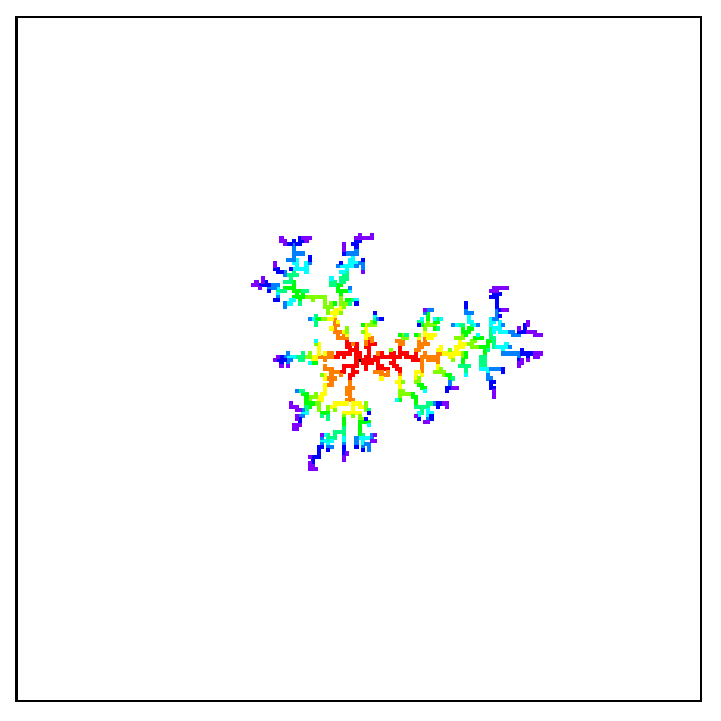
\includegraphics[width=8.0cm]{figure_2.pdf}
                        \caption{$N=1000$の時に得られたDLAクラスター.$N$の100個ごとに色を変えてある.}
                        \label{fig:14-9-f1}
                    \end{center}
                \end{figure}
                
            \end{enumerate}    
        
        \item $t=0$で,正方格子の4個の周辺(成長)点はおのおの成長確率,すなわち,クラスタの一部となる確率$p_{i}=1/4$を持っている.$t=1$では,そのクラスターの質量は2となり,6個の周辺の点を持つことになる.どの格子点が周辺の点になるか理解し,それらの成長確率は一定でないことを確認せよ.モンテカルロ・シミュレーションを行い,2つの周辺の点については$p_{i} =2/9(= 0.222\cdots)$であり,他は$p_{i}= 5/36(= 0.13888\cdots)$であることを確かめよ.問題14.10で成長確率を決定する更に直接な方法について議論する.
        
            \begin{enumerate}
                \item $t=1$では,図\ref{fig:14-9-f2}に示したように6個の周辺の点をもっている.3000回の試行によるモンテカルロ・シミュレーションで,図のそれぞれの位置に粒子が付着する確率確率$p, q, r, s$を求めた.結果は$p = 0.141,q = 0.1375, r = 0.22166666666666668, s =  0.22133333333333333$であった.すなわち,2つの粒子に対して,クラスターの長さが長くなるような位置に,粒子が付着しやすいということがわかった.これは,得られたクラスターの形からも確かめられることであり,クラスター成長していくときに,その形を丸くするようにではなく,細長く伸びていくような成長の仕方をしていることも観察できている.
                
                ここで,$p,q,r,s$の判別について述べておくこととする.中心の点と周囲1マスの計9個の格子点で作られる格子を考える(図\ref{fig:14-9-f2}の赤枠で囲まれた格子点).まず,その格子内の粒子数が2であるものは$r$であると分かる.次に,中心の点の上下左右の4点の粒子数の和が1となるのは粒子が$p$で付着する場合のみである.最後に,行方向と列方向で和を計算し,その値に3が含まれているのは$s$のときのみであるので,これで$s$と$q$を区別することができる.$p$と$q$に対しては,二通りの付着の仕方が考えられるため,2で割る必要があり,このようにしてそれぞれの付着確率$p,q,r,s$を求めることができた.
                
                \begin{figure}[H]
                    \begin{center}
                        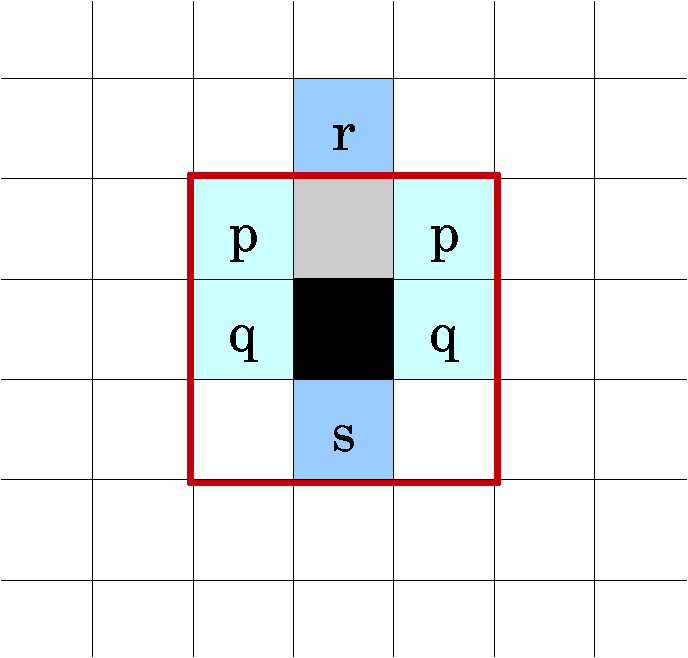
\includegraphics[width=8cm]{figure_3.pdf}
                        \caption{$t=1$における6つの周辺の点.}
                        \label{fig:14-9-f2}
                    \end{center}
                \end{figure}
                
            \end{enumerate} 
        
            \item クラスターの周辺の点から遠く離れたところでのランダムウォークにCPU時間のほとんどが費やされてしまうので,DLAクラスターの生成に使用しているプログラムは能率的ではないだろう.この問題を克服するための方法がいくつかある.1つの方法はランダムウォークの歩幅をクラスターから離れるにしたがって大きくすることである.たとえば,粒子が距離$R>R_{\mathrm{max}}$にいて,$R-R_{\mathrm{max}}-1$が単位の格子間隔よりも大きいならば,この距離に等しいかそれ以上の歩幅を許すことにする.粒子がクラスターに非常に近い場合は,歩幅を単位の格子間隔にとる.他の可能な修正についてミーキン(Meakin)による議論がある\cite{Meakin1993189}.自分のプログラム(あるいは教科書\cite{textbook}にあるプログラムdie)を修正し,正方格子上の2次元の拡散律速クラスターのフラクタル次元を求めよ.
        
            \begin{enumerate}
                \item ランダムウォークの歩幅が,中心からの距離$r$が大きくなるほど大きくなるように変更を加え,クラスターより遠い位置でのランダムウォークに費やす時間が出来るだけ小さくなるようにプログラムを変更した.得られた拡散律速クラスターのフラクタル次元を,視野拡大法によって求めた.$N=1000$として視野のスケール$b$とその範囲内の粒子数$M(b)$の関係を両対数グラフに表し,その傾き$D$を求めた.これを図\ref{fig:14-9-f3}に示す.傾き$D$は$D=1.616042$と求められた.
                
                \begin{figure}[H]
                    \begin{center}
                        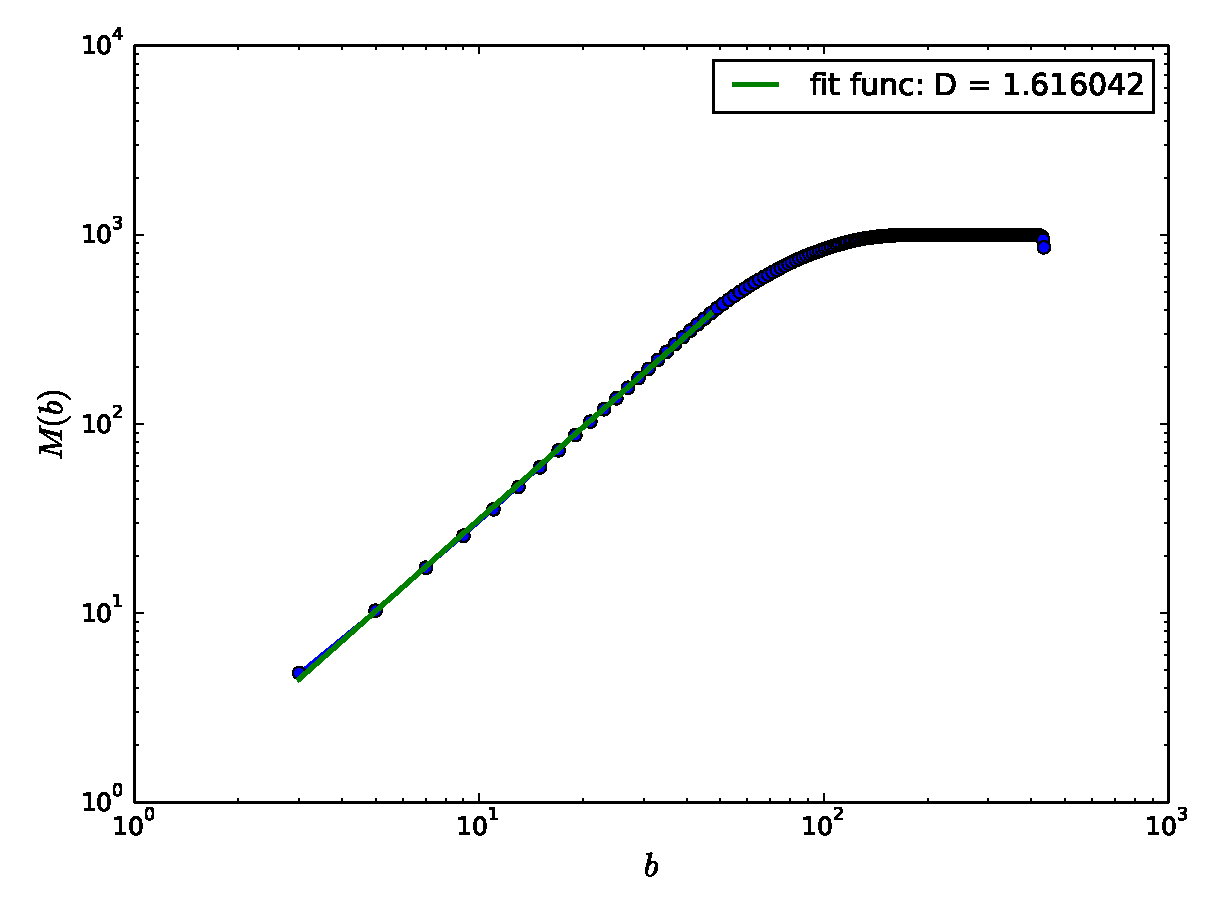
\includegraphics[width=10cm]{figure_4.pdf}
                        \caption{$N=1000$のとき,得られたDLAクラスターのフラクタル次元.}
                        \label{fig:14-9-f3}
                    \end{center}
                \end{figure}
                
            \end{enumerate}
    \end{enumerate}

\section{まとめ}
    自然界の様々な場所で見られるパターンの基本的なモデルである,拡散律速凝集のクラスターについて理解することができた.見ただけでフラクタル次元が正確に予想できるようになるまで精進できればと思う.


\bibliography{/home/shotaro/Workspace/computing_simulation/reference}

\end{document}
